\documentclass[12pt]{article}
\usepackage[utf8]{inputenc}
\usepackage[margin=1in]{geometry}
\usepackage{float}
\usepackage{graphicx}
\usepackage{physics}
\usepackage{amsmath}
\usepackage{amssymb}
\usepackage[colorlinks]{hyperref}
\usepackage{subcaption}
\captionsetup{font=footnotesize}
\usepackage{booktabs}
\usepackage{multirow}
\newcommand{\otoprule}{\midrule[\heavyrulewidth]}
\usepackage[export]{adjustbox}
\bibliographystyle{plain}
\title{Final Report on Summer Internship \\
\large{Unstable Electron Flow in a Corbino Disk}}
\author{Jack H. Farrell \\ \small Supervisors: Prof. Nicolas Grisouard, Prof. Thomas Scaffidi}

% End Preamble, Begin Document
\begin{document}
	
%%% ABSTRACT ----------
\begin{abstract}
According to recent simulations, compressible, viscous electron flow through a straight channel can undergo an instability that terminates as a coherent nonlinear oscillator.  The oscillatory behaviour shows promise as a source of radiation that could fill the so-called TeraHertz gap, a region of the electromagnetic spectrum for which no good sources or detectors exist.  We describe a computational study of this same \textit{Dyakonov-Shur Instability} in a different setup; we modeled the radial flow of viscous electrons in a Corbino disk.  Our simulations show that the endpoint of the instability is still a coherent nonlinear oscillator in this new geometry, and we also notice that annular devices can enhance the prevalence of the instability and its radiated power while decreasing the frequency.  In particular, in an annular device, the instability can exist at somewhat stronger momentum relaxation than the straight-channel device. 
\end{abstract}

%\keywords{Suggested keywords}%Use showkeys class option if keyword
                              %display desired
% Title
\maketitle

% Table of Contents
\tableofcontents

%%% INTRODUCTION ----------
\section{Introduction}
Theoretically, when the size of a system is much larger than the mean free path of electron-electron interactions while still somewhat smaller than that of electron-phonon and electron-impurity interactions, the electron gas can be described well by hydrodynamic equations.  Recent experiments in Graphene have made this interesting regime seem more approachable, meaning an old hydrodynamic mechanism for the generation of TeraHertz radiation proposed by Dyakonov and Shur~\cite{Dyakonov1993} may prove useful.  

Currently, the electromagnetic spectrum contains a ``TeraHertz Gap" around $10^{12}\ \text{Hz}$, meaning there are not effective sources or detectors of radiation in this range.  Dyakonov and Shur~\cite{Dyakonov1993} studied the hydrodynamic equations in the setting of a Field Effect Transistor (FET) subject to some unusual boundary conditions, and they noticed that the flow is unstable: small perturbations to the steady state do not decay, and those growing modes in fact have oscillation frequencies in the TeraHertz range.  Recently, some simulations performed by Mendl, Polini, and Lucas~\cite{Mendl2019} have made the instability seem even more promising as a radiation source, since they found that the growing oscillations reach a finite amplitude and that the system terminates as a \textit{coherent nonlinear oscillator}.  

In addition, the performance of FETs has been found to depend on their geometry.  For instance, the Dyakonov-Shur Instability has been investigated in cylindrical FETs and Corbino disk FETs~\cite{Li2019}~\cite{Sydoruk2010}.  

We pursue the latter option, motivated by some promising results about the converse problem of TeraHertz detectors~\cite{Khavronin2020}.  That is to say, we model current-driven radial flow in a Corbino disk.
For our simulations and even the linear analysis, we work mostly in a regime that is very close to the straight channel studied in~\cite{Mendl2019}.  In these setups that have large radii compared to the separation of the two rings, we find that the instability exists at lower bias velocities than the rectangular case; in other words, the geometry enhances the instability.

In this report, we establish our model and summarize some of the promising results that speak to the favour of Corbino FETs.



%%% MODEL ----------
\section{\label{sec:model}Model\protect}

We model electrons, charge $-e$ and mass $m$, in the annulus $a < r < b$. We also imagine applying a steady (not necessarily uniform) radial electric field $\vb{E} = E(r)\vu{r}$.  The electrons are described by their number density $n(r, t)$ and momentum density $J(r,t)\equiv n(r,t)v(r,t)$, where $v(r,t)$ is their velocity field.  We assume both are radially symmetric; in other words, the flow only has a component in the radial direction, and, moreover, it only depends on the radial coordinate $r$. The assumption of radially symmetric flow, which leads to an effectively one-dimensional model, is justified by the radial symmetry of the boundary conditions~(\ref{eq:BCs}), as we shall see, and also by the fact that azimuthal modes would not couple to the radial electric field.

Motivated by~\cite{Mendl2019}, we impose the unusual boundary conditions known as \textit{Dyakonov-Shur Boundary Conditions}, fixing the mass at $n_0$ on one end of the channel and the momentum at $n_0 v_b$ on the other:
\begin{subequations}
	\label{eq:BCs}
	\begin{eqnarray}
	J(b)&=&J_b\equiv n_0v_b, \label{eq:bc1}
	\\
	n(a) &=& n_0, \label{eq:bc3}
	\\
	\left.\pdv{r}(rJ)\right|_{r=a} &=& 0. \label{eq:bc2}
	\end{eqnarray}
\end{subequations}

Completing the model requires accounting for a few more effects.  First, we call the thermodynamic pressure $P(n)$.  In addition, electrons in this regime will experience both viscosity and momentum relaxation.  To measure these effects, let $\eta$ be the coefficient of dynamic viscosity and $\gamma \equiv 1/\tau$ be the momentum relaxation rate.  With the boundary conditions noted above, it is useful to write the electric field $E$ in terms of the steady state of DC current it generates.  Assuming a constant equilibrium charge density $n_0$ and neglecting the nonlinear advection term, the steady state velocity field must be $v_0(r) = b v_b / r$ in order to satisfy the continuity equation in cylindrical coordinates and the boundary condition~(\ref{eq:bc1}).  Then, the Newton's Law balance implies a steady state as long as $E(r)$ has $1/r$ dependence, giving:
\begin{equation}\label{eq:E}
\frac{-e}{m} E(r)=v_0(r) = \gamma \frac{b v_b}{r}.
\end{equation}
We model the dynamics near this steady state using the nonlinear hydrodynamic equations:

\begin{subequations}\label{eq:mainEquations}
\begin{eqnarray}
\pdv{J}{t}+\frac{1}{r}\pdv{r}(\frac{rJ^2}{n}) + \frac{1}{m}\pdv{P(n)}{r} -  \frac{\eta}{m}\left(\laplacian-\frac{1}{r^2}\right) \frac{J}{n}
&=& \gamma\left( n\frac{bv_b}{r} - J\right), \label{eq:momentumEquation}
\\ 
\pdv{n}{t} + \frac{1}{r}\pdv{r}(rJ) &=& 0. \label{eq:massEquation}
\end{eqnarray}
\end{subequations}
Here,$\laplacian \equiv \pdv[2]{r} + \frac{1}{r}\pdv{r}$ is the scalar laplacian operator.  For the pressure $P$, we take the simplified ideal gas equation of state $P(n) = mv_s^2n$, where $v_s$ is the density-independent speed of sound.



Finally, to make the relationship with the rectangular geometry more clear, we define $L \equiv b - a$ to be the channel length.  Then, as we let $L / a \rightarrow 0$, Eq.~(\ref{eq:mainEquations}) reduces to the equations describing viscous electrons in a straight channel.  As such, we use the quantity $L/a$ as a measurement of the difference between the rectangular geometry and our corbino disk geometry.

According to linear theory, perturbations to the steady state should have complex frequencies of the form:
\begin{equation}
\label{eq:linear}
    \omega_l = \frac{\pi v_s}{2L} + \mathrm{i}\left(\frac{v_0}{L}\left(1 + \frac{L}{a}\right)-\frac{\gamma}{2}-\frac{\nu\pi l^2}{8 L^2} \right) + \ldots,
\end{equation}
where $l = 1, 3, 5, \ldots$ is the mode number.  Note that we show only terms that are first order in the parameters $v_0$, $\nu$, $\gamma$, and $L / a$.  Whenever the imaginary part of the $l = 1$ mode is positive, the instability should exist, so we expect from Eq.~(\ref{eq:linear}) that the instability should be more prevalent when $L/a$ is higher.  Note that one is not limited to first order in $L/a$ --- the linearized equations can be solved in general using numerical techniques.  The numerical solution to the eigenvalue problem agrees well with Eq.~(\ref{eq:linear}), so in the rest of this report, when comparing to the predictions of linear theory, we show the results of Eq.~(\ref{eq:linear}).



%%% SIMULATIONS ----------
\section{\label{sec:simulations}Simulations\protect}

We used finite volume methods to solve Eq.~(\ref{eq:mainEquations}) numerically. Our main finding is that the corbino geometry favours the existence of the instability as compared to the rectangular geometry --- in the annulus, the instability can exist in some regions of $v_b, \eta, \gamma$ parameter space where did not in a straight channel.  Like in the rectangular geometry, we observe the endpoint of the instability to be a coherent nonlinear oscillator for which neither the frequency nor the amplitude depend on the initial conditions.  In quoting results from the simulations, it is useful to work in terms of the following non-dimensional scalings of the parameters $v_b$, $\eta$, $\gamma$: $\tilde{v_b}\equiv v_b/v_s$, $\tilde{\eta} \equiv \eta/n_0 m v_s L$, $\tilde{\gamma} \equiv \gamma L / v_s$.

To start, Fig.~(\ref{fig:illustration}) shows the behaviour of $n(b, t)$ (the density at the opposite end of the device from where it is fixed by the boundary conditions). The parameters $v_b$, $\eta$, and $\gamma$ were chosen so that if $L / a$ is small (geometry is almost rectangular), the instability does not exist--- the small perturbation to $n_0$ decays over time.  But at $L/a=0.5$, a channel length that is one half the length of the inner radius, the $n(b,t)$ trace grows and reaches a limit cycle with fixed amplitude and a well defined period $T$. 
\begin{figure}[ht]
	\centering
    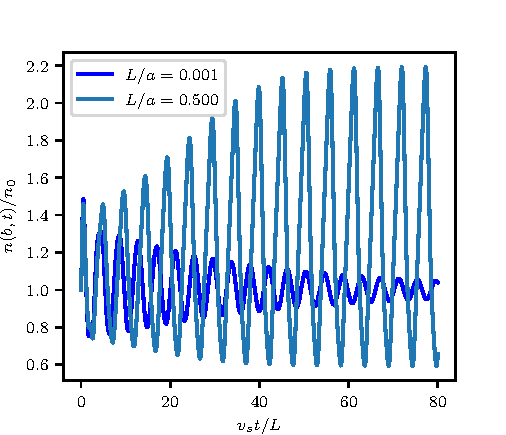
\includegraphics{Figures/illustration.pdf}
    \caption{Oscillation of $n(b, t)$ for a choice of parameters $\tilde{v_b}=0.07$, $\tilde{\eta}=0.03$, $\tilde{\gamma}=0.1$.  When $L/a = 0.001$, corresponding to the rectangular geometry, the $n(b,t)$ trace decays.  For $L/a=0.5$, the instability exists.}
    \label{fig:illustration}
\end{figure}


%%% (Might delete this section? NOt sure if need to show snapshots)
%For the same parameters, Fig.~(\ref{fig:snapshots}) shows snapshots of the $n$ and $J$ fields over the period of the nonlinear oscillator.  As in the rectangular geometry, the snapshots show a shock wave moving to the left and a rarefaction wave moving to the right.

We now describe more thoroughly the dependence of the onset of the instability, its frequency, and it's amplitude on $L/a$ and the parameters $v_b$, $\eta$, and $\gamma$.  To start, Fig.~(\ref{fig:v0_ratio}) gives the frequency as a function of $v_b$ and $L/a$.  
\begin{figure}[ht]
	\centering
	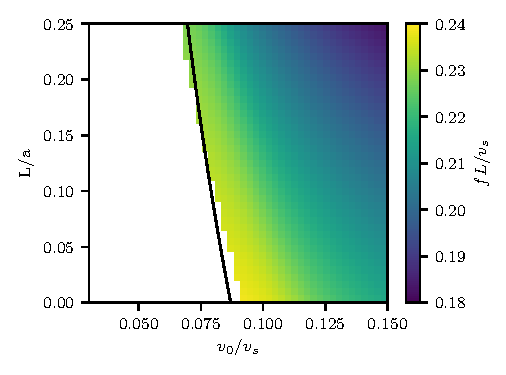
\includegraphics{Figures/v0_ratio1.pdf}
	\caption{The frequency of the nonlinear oscillator as a function of $v_b$ and $L/a$.  Where the plot is white, the instability does not exist. The black curve denotes the boundary between stability and instability as predicted by the linear theory --- left of the curve should be stable; right of the curve, unstable.  The parameters were $\tilde{\eta}=0.03$ and $\tilde{\gamma}=0.1.$}
	\label{fig:v0_ratio}
\end{figure}
Increasing $L/a$, which makes the geometry more disk-like, allows the instability to exist at lower $v_b$. Similarly, Fig.~(\ref{fig:v0_ratio_power}) shows that increasing $L/a$ also raises the amplitude of the nonlinear oscillator.
\begin{figure}[ht]
	\centering
	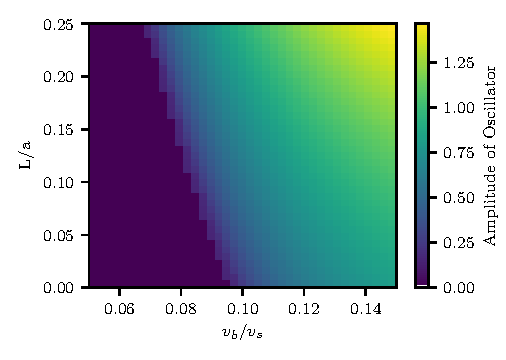
\includegraphics{Figures/v0_ratio_power1.pdf}
	\caption{The amplitude of the nonlinear oscillator as a function of $v_b$ and $L/a$.  The parameters were $\tilde{\eta}=0.03$ and $\tilde{\gamma}=0.1.$}
	\label{fig:v0_ratio_power}
\end{figure}
As we will see, the ampliude of the oscillator strongly affects the amount of power the device can radiate.

We can see the same effect, that increasing $L/a$ allows the instability to exist at smaller $v_b$, by comparing the dependence of the instability on $v_b$ and $\eta$ in different setups.  We show an example in Fig.~(\ref{fig:v0_eta}), which gives the frequency as a function of $v_b$ and $\eta$. 
\begin{figure}[ht]
	\centering
	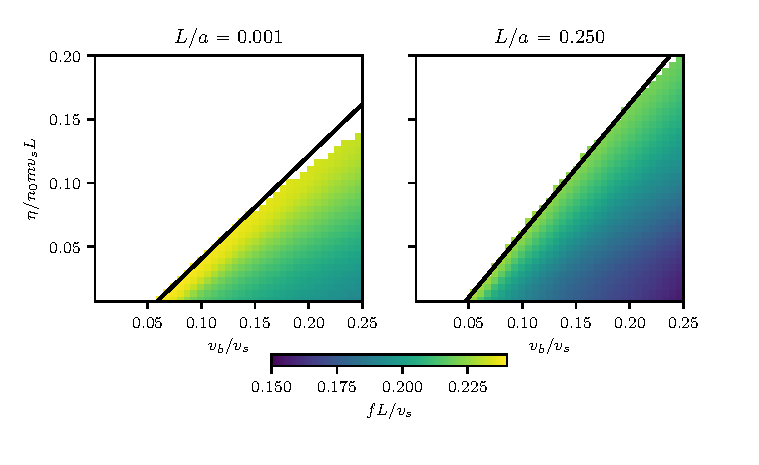
\includegraphics{Figures/v0_eta_freq.pdf}
	\caption{Frequency and existence as a function of $\eta$ and $v_b$ for two different geometries.  Where the graph is white, the instability does not exist.  The black curve gives the boundary between stability and instability as predicted by Eq.~(\ref{eq:linear}) --- to the left of the curve, the system should be stable; to the right, unstable.  We fixed $\tilde{\gamma} = 0.1$.}\label{fig:v0_eta}
\end{figure}
Notice that when the geometry is more circular, corresponding to $L/a = 0.250$ as compared to $0.001$, the slope of the boundary between the stable and unstable region is steeper, and the boundary has also been slightly translated toward lower $v_b$.  The plot means that with the same fixed drift velocity $v_b$, the instability can persist to higher viscosity when the device is disk-shaped than when it is rectangular. 



It is important to note some of the problems we encountered while simulating Eq.~(\ref{eq:mainEquations}).  That discussion can be found in Appendix~\ref{sec:problems}.


%%% APPLICATIONS ----------
\section{Applications}
In this section, we discuss the prospects of devices with the Corbino geometry in terms of generating TeraHertz radiation. 


\subsection{Current or Current Density?} 
To start, we note that it is easy to misinterpret Fig.~(\ref{fig:v0_ratio}).  Hidden so far is the important fact that changing $L/a$ also changes the dimensions of the device --- for instance, at fixed $L$, to raise $L/a$ we would need to make $a$ and $b$ smaller.  The size of the sample in turn determines the amount of power the device can produce.  Further, the parameter $v_b$ is proportional to a current \textit{density}, meaning that for larger $b$ and fixed $v_b$, the device would need to draw more \textit{current}.  In that way, for a fixed $L$, making the device more and more circular may not be more favourable than straight-channel-detectors.

In this paragraph, we make some arguments as to why, in the first place, the ability to produce the instability at lower current \textit{density}, $v_b$, is still useful.  First, one limitation of field effect transistors is that the velocity of the charge carriers tends to ``saturate" at high external electric fields $E$.  In those cases, it is really high velocities, not necessarily currents, that prove challenging experimentally.  The ability to reach the instability with lower carrier velocities, then, could be a desirable feature in terms of creating a a real device --- one could use a material with somewhat smaller \textit{electron mobility}.  Secondly, related to the above, we also notice that the applied electric field $E$ could have lower magnitude than in the corbino case --- by Eq.~(\ref{eq:E}), the minimum value of $E(r)$ over the whole channel will be proportional to $v_b$\footnote{Informal note from Jack: I am having trouble finding a reference for this next point --- I may check with some friends who have worked in some labs that spend time with these small-scale electronics.  But there is a sentence in~\cite{Mendl2019} that reads ``...such bias current is accessible experimentally without undue heating of the phonons". To me, it would be very surprising if a it were high \textit{currents} that mattered for ``undue heating of the phonons" more than current density.  Surely, a small device (higher current \textit{density} for same \textit{current}) would be more prone to phonon heating than a large device.  That is what makes me think the current density may be the better figure of merit here... basically, I'm trying to argue that the microscopic issues that limit the effectiveness of a field effect transistor care more about the density of the current than the current itself.} \footnote{Another informal note: Additionally, I do not believe it is a coincidence that~\cite{Mendl2019} use measure like $v_b$ rather than current $I$.  It really could be that the currents we are talking about are pretty small anyway, so reaching the currents we need is not so hard - but there are issues with fixing the charge density at a certain point.  (If you think about it, if current were a huge issue, you could just use a device of slightly smaller $W$, and just live with losing a little bit of power.  In fact, you will lose power anyway if you reduce the current in the device.)}.

Nonetheless, it would still be interesting to know if the corbino geometry would after all allow the instability to exist at lower current \textit{I} without losing power radiated. In other words, if we \textit{did} have a disk-shaped device that drew the same amount of current as a rectangular device, how would the radiated power compare? As a specific example, consider a device intended to generate radiation of frequency $f=1.5\ \text{THz}$.  By Eq.~(\ref{eq:linear}), the channel length should be roughly $L = 0.2\ \mu\text{m}$.  Suppose the outer cylinder has a circumference $2 \pi b = 7\ \mu\text{m}$.  For this, $b$ would be $1.11 \ \mu\text{m}$.  Then, $a = b - L$ would then need to have length $a = 0.9\ \mu\text{m}$, leading to $L/a = 0.22$.  Consider as well an analagous rectangular device, which has the same value for $L$ and also a $W$, the width, equal to the outer circumerence, $W = 7\ \mu\text{m}$.  In this case, the bias current density $\tilde{v_b}$ really \textit{does} correspond to the exact same current \textit{I} in each case.  We can already notice from Fig.~(\ref{fig:v0_ratio}) and Fig.~(\ref{fig:v0_ratio_power}) that the Corbino device at these parameters is deeper in the unstable regime --- the oscillations will have higher amplitude at the same $I$, and the instability could exist at lower $I$ in the first place if that were desirable.

To go further in the comparison, it helps to work out an upper bound on the radiated power directly.  In the rectangular case, this upper estimate of the power can be calculated as:
\begin{equation}
\label{eq:rectPower}
P = \frac{1}{T}\left| \frac{1}{T}\int_t^{t+T} \frac{1}{2C}Q^2(t)\cos(\frac{2 \pi t}{T}) \mathrm{d}t\right|,
\end{equation}
where $C = \epsilon_0\epsilon_{zz}A / d$ is the geometric capacitance.  $A$ is the area of the capacitor, given by $A = LW$ in the rectangular case and $A=\pi(b^2-a^2)$ for the annulus.  The charge $Q(t)$ is found by integrating the charge density $n$:
\begin{equation}
\label{eq:rectCharge}
Q(t) = -eW  \int_0^Ln(x,t) \mathrm{d}x.
\end{equation}
However, in the corbino case, we can still use Eq.~(\ref{eq:rectPower}), but the expression for the charge $Q(t)$ should instead be:
\begin{equation}
\label{eq:rectCharge}
Q(t) = -2 \pi e\int_a^b r n(r,t)\mathrm{d}r.
\end{equation}

Using Eq.~(\ref{eq:rectPower}), we upper-bound the power radiated in the rectangular device as $4.1\times 10^{-6}\ \text{W}$ and that in the corbinio geometry as $62.3 \times 10^{-6} \ \text{W}$.  At the same time, the frequency decreases from 1.6 THz to 1.3 THz when the geometry is changed from rectangular to corbino.  In the next paragraph, we give one interpretaion of this striking behaviour.  But for now, we note that if the goal is to generate more power, one should aim to be as far in the unstable region of parameter space as possible --- and the Corbino geometry can help accomplish this.




\subsection{Interpretation of L/a Behaviour}
One interpretation of the effect switching to an annular geometry is motivated by Eq.~(\ref{eq:linear}). So long as it is small, the parameter $L/a$ enters the equation by effectively raising $v_b$.  In fact, even outside of this equation, the system behaves according to the interpretation that the bias current $v_b$ is ``geometrically enhanced".  For instance,~\cite{Mendl2019} observed, numerically, that increasing the bias current decreases the frequency while raising the radiated power, which is precisely the behaviour we notice with increasing $L/a$. But using a disk-shaped device to raise the power instead of the current may be an easier prospect experimentally.

\subsection{Higher-Order Effects of Corbino Geometry}
We also, however, observe some effects from the Corbino geometry that go beyond the interpretation of Eq.~(\ref{eq:linear}) given above.  One important example is that the Corbino geometry can overcome greater momentum relaxation than the rectangular case.  In the rectangular geometry, as noticed in~\cite{Mendl2019}, the presence of momentum relaxation poses major difficulties in terms of observing the instability experimentally --- in particular, past a certain critical value of $\gamma$, the instability does not exist at \textit{any} value of $v_b$.  Our work in the corbino geometry shows the same feature --- however, even at modest values of $L/a$, we observe the critical $\gamma$ to be higher in the corbino geometry.  This important fact, illustrated in Fig.~(\ref{fig:v0_gamma}), suggests corbino field effect transistors may yield easier detection of this instability.
\begin{figure}[ht]
	\centering
	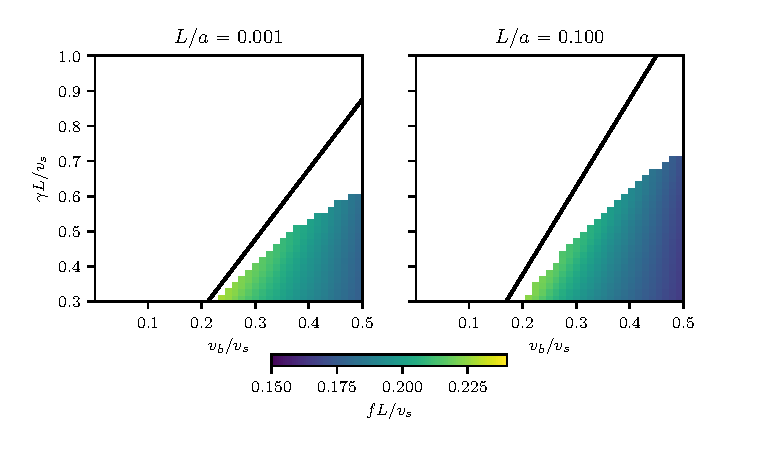
\includegraphics{Figures/v0_gamma0_freq.pdf}
	\caption{Frequency and existence as a function of $\gamma$ and $v_b$ for two different geometries.  Where the graph is white, the instability does not exist.  The black curve gives the boundary between stability and instability as predicted by Eq.~(\ref{eq:linear}) --- to the left of the curve, the system should be stable; to the right, unstable.  We fixed $\tilde{\eta}=0.05$.}\label{fig:v0_gamma}
\end{figure}
Note that, in Fig.~(\ref{fig:v0_gamma}), the black curve summarizing the linear theory does not fit the numerical results well.  This result is not unexpected, since the values of $\gamma$ and $v_b$ are \textit{not} small over the range shown in the figure.

\section{Conclusion}
On several levels, then, our simulations suggest that FETs shaped like Corbino disks could prove more effective than their rectangular counterparts in terms of generating radiation.  Firstly, they allow the instability to exist at lower fixed current densities, a property that could be desirable experimentally.  Second, even if the fixed drift velocity / current density is not so useful, one can imagine Corbino Disks with circumference corresponding to a sample width in the rectangular case, and we have seen that such devices should emit more power at the same fixed current.  Finally, the critical value of momentum relaxation is higher for Corbino devices than for straight channels, a property independent of the confusion surrounding the parameter $v_b$.

To us, three main future directions seem promising for related work.  Firstly, in the Corbino Geometry, some other boundary conditions may prove useful.  Calculations at the beginning of the decade~\cite{Sydoruk2010} found that \textit{symmetric} boundary conditions (for instance, fixing the momentum at both boundaries or fixing the density at both boundaries) could still lead to an instability in the Corbino case.  By contrast, these boundary conditions \textit{never} yield an instability in the case of a straight channel.  One big reason to want to use symmetric boundary conditions is that the fundamental frequency is double that of the current asymmetric situation.  Observing the endpoint of this uniquely Corbino instability through simulations would be useful.

Secondly, in the annulus, one could consider driving angular modes in the system using an external magnetic field $\vb{H}$ directed along the $\vu{z}$ axis.

Finally, one could look to simulate hydrodynamic situations even outside the Dyakonov-Shur Instability.  The Navier-Stokes equations allow many interesting phenomena; one could consider the electronic analogues of phenomena like, for instance, Lee waves (what happens viscous electrons are sent over a periodically-varying ``bottom surface"?).
 



\bibliography{../../../../Bibliographies/final_report}{}

% The \nocite command causes all entries in a bibliography to be printed out
% whether or not they are actually referenced in the text. This is appropriate
% for the sample file to show the different styles of references, but authors
% most likely will not want to use it.

\appendix
\section{Numerical Method}
Take the equations \ref{eq:mainEquations} without the relaxation term and the viscous term, i.e., $\gamma = 0$ and $\eta = 0$.  The remaining terms can be put in the following form:
\begin{equation}
\label{eq:conservationLaw}
\renewcommand\arraystretch{3}
\pdv{t}
\begin{pmatrix}
n \\
J
\end{pmatrix}
+ \pdv{r}
\begin{pmatrix}
J \\
\dfrac{J^2}{n} + v_s^2n
\end{pmatrix}
=
\begin{pmatrix}
\dfrac{-J}{r} \\
\dfrac{-1}{r} \dfrac{J^2}{n}
\end{pmatrix}.
\end{equation}
The left-hand-side of this equation is equivalent to the \textit{isothermal equations} from gas dynamics in one spatial dimension.  The right-hand-side represents additional source terms from the corbino geometry (``geometric source terms").  

For the left-hand-side of~(\ref{eq:conservationLaw}), which is called the \textit{conservation part} of the equation, we use finite volume methods.  In particular, we use Roe's Approximate Riemann Solver with a slope limiter (we choose the \texttt{minmod} limiter) to make a high-resolution method.  The simulation has a spatial step width $h=1/50$ and a temporal step width $k = 0.0005$.

The viscous term is incorporated into the above \textit{conservation step} of our solution by using the centered finite-differences approximations to the derivatives.  For the vector laplacian in polar coordinates, this looks like:
\begin{equation}
\frac{1}{r h} \left( \left(r + \tfrac{h}{2}\right)\frac{q(r+h)-q(r)}{h} - \left(r-\tfrac{h}{2}\right)\frac{q(r)-q(r-h)}{h}  \right) -\frac{q}{r^2},
\end{equation}
where $q \equiv J/n$.  Note that the last term, which has no derivatives, could just as well have been incorporated into the other step of the simulation, which is described in the next paragraph.

Finally, for the relaxation term and the geometric source terms (right-hand-side of Eq.~(\ref{eq:conservationLaw})), we use an operator splitting method called \textit{Strang Splitting}.  In this approach, we start by integrating a half time step $k/2$ pretending the equation is $\pdv{J}{t} =  \text{relaxation term} + \text{geometric source terms}$.  We use the result of that as initial conditions for the conservation step, and perform a full time-step $k$.  Then, we use the result of \textit{that} as initial conditions for another half time step of source terms and relaxation.  

\section{Limitations of Simulations}
\label{sec:problems}
We found that for higher $L/a$ than reported in the main text, the numerical method ``blew up".  It would be good if future work could probe this ``highly annular" regime more carefully.  We suppose the problem in the method could be just that the shocks become too strong --- some more numerical viscosity may be needed to capture them.  This could be accomplished by tuning some parameters in the numerical method that have to do with something called an \textit{entropy fix}, but one would have to be careful that the amplitude and frequency of the oscillator do not depend too strongly on these parameters before increasing them to reach a more annular regime.

Still, the good agreement with linear theory at relatively low $L/a$ suggests that the numerical method is converging to the right solution as long as it is correctly capturing the shocks.
 


 
\end{document}